\section{Description of Alternative 5-D Initial Density}
In Figure~\ref{fig:pde-highd-2d-scatter}, we plot the initial samples which have normalized ratios densities associated with $\qoi_{1D}$ and $\qoi_{2D}$ and remark that the scalar--valued QoI map identifies a contour which appears to trace a straight line through $\pspace$.
This can be helpful for identifying the correlation structure and defining a lower-dimensional subspace to perform rejection sampling However, the solution that comes from using $\qoi_{2D}$ is better at reducing uncertainty.
Taken together, these observations can be used to suggest a number of sampling strategies to generate a new initial density.
We propose one such approach here.

\begin{figure}[htbp]
\centering
  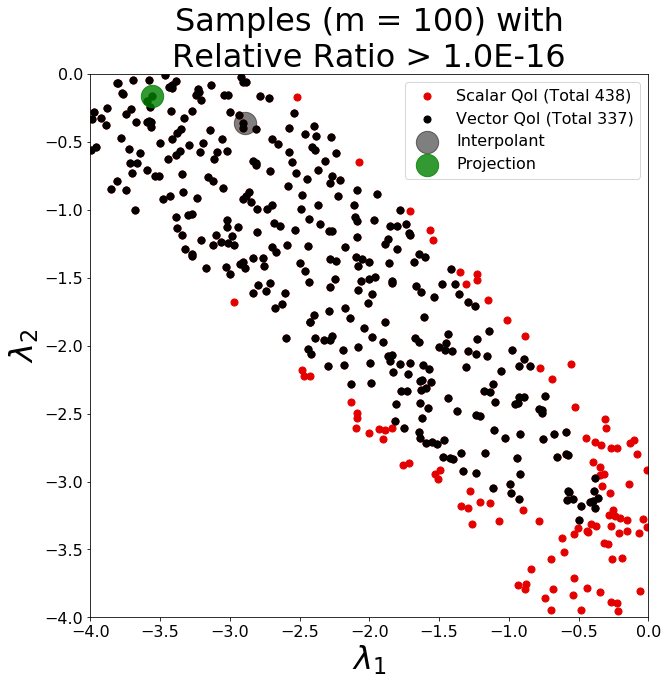
\includegraphics[width=0.45\linewidth]{figures/pde-highd/pde-highd_update_scatter_D2_t1-0E-16.png}
  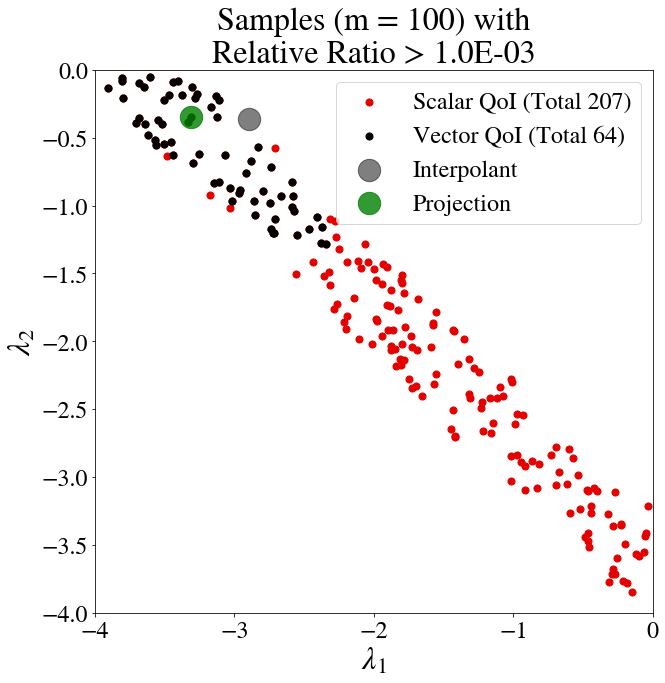
\includegraphics[width=0.45\linewidth]{figures/pde-highd/pde-highd_update_scatter_D2_t1-0E-03.png}
\caption{
100 measurements
}
\label{fig:pde-highd-2d-scatter}
\end{figure}


\begin{figure}[htbp]
\centering
  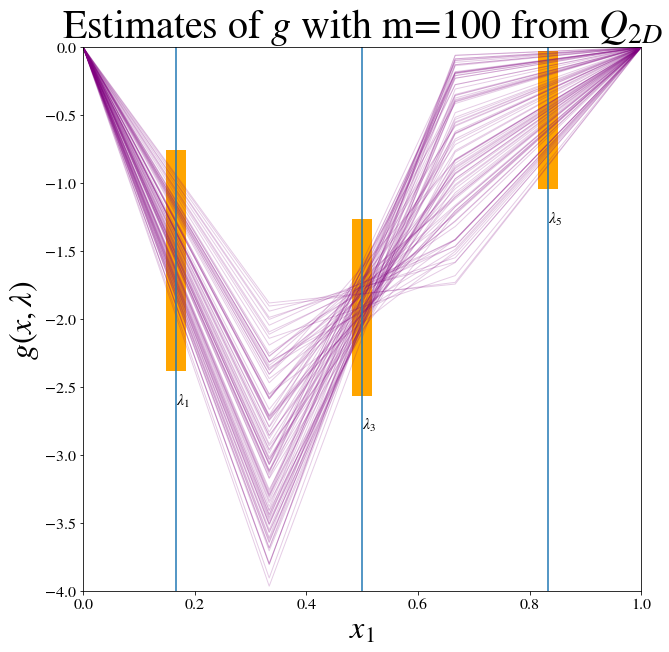
\includegraphics[width=0.675\linewidth]{figures/pde-highd/pde-highd-alt_initial_D5_m100.png}
\caption{
Knowledge of the behavior of $g$ at the boundaries allows for more than half of each of the three remaining intervals in five dimensions to be ruled out as infeasible regions when we look at high-probability samples from the 2-D SIP solution.
}
\label{fig:pde-highd-5d-study}
\end{figure}

In Figure~\ref{fig:pde-highd-5d-study}, we plot the parameter samples whose relative ratios exceeded $1/1000$ and note that they sweep out a family of curves that can be used to estimate bounds not only on $\lambda_2$ and $\lambda_4$ (the previous $\lambda_1$ and $\lambda_2$ from the 2-D problem)\---which exhibit correlation structure\---but also on the remaining three knots.
To form the intervals shown in orange in Fig.~\ref{fig:pde-highd-5d-study}, we take the upper and lower bounds of the curves passing through the vertical lines drawn at the three new knot values.
To be conservative, we multiply our lower bound by $1.2$ and the upper by $0.8$.
With these choices, we are still more than halving the interval-length in each direction as compared to the previous 5-D problem.
One could establish a lower tolerance for accepting likely samples and avoid the multiplication factor, or make any number of other choices for a refined initial density.
However, a thorough exploration of how to best leverage the ratio of observed to predicted densities is left to future work, and will always be highly problem--dependent.


\subsection{Capturing Correlation Structure from 2-D SIP Solution}
For the two remaining directions, we want to capture the correlation structure that we were able to visually identify in Fig.~\ref{fig:pde-highd-2d-scatter} and impose a uniform density over the support of the set.
To achieve this desired refinement of an initial density, we perform a singular-value decomposition on the likely samples from the scalar--valued 2-D solution, since there are so many more samples\footnote{ The scalar-valued contour was found to better characterize the direction of the equivalence class, suggesting perhaps a justifiable use for solving the problem with it. We could have formed an estimate of the updated density from using the vector--valued QoI and sampled from that instead. Many such approaches can be looked into in the future and are briefly discussed in the last section of this chapter.}.
The singular vectors are used to transform the vector-valued samples, and a uniform sampling is performed over the rectangular bounding box for these points, shown in the center of Figure~\ref{fig:pde-highd-2d-study}.
These generated samples, however, leave $\pspace$ when transformed back to their native space, as seen in the left panel.
To ameliorate this problem, we instead perform sampling in a while-loop, sampling from this uniform box and rejecting any that would get mapped back outside $\pspace$, until we reach our desired thousand samples.


\begin{figure}[htbp]
\centering
  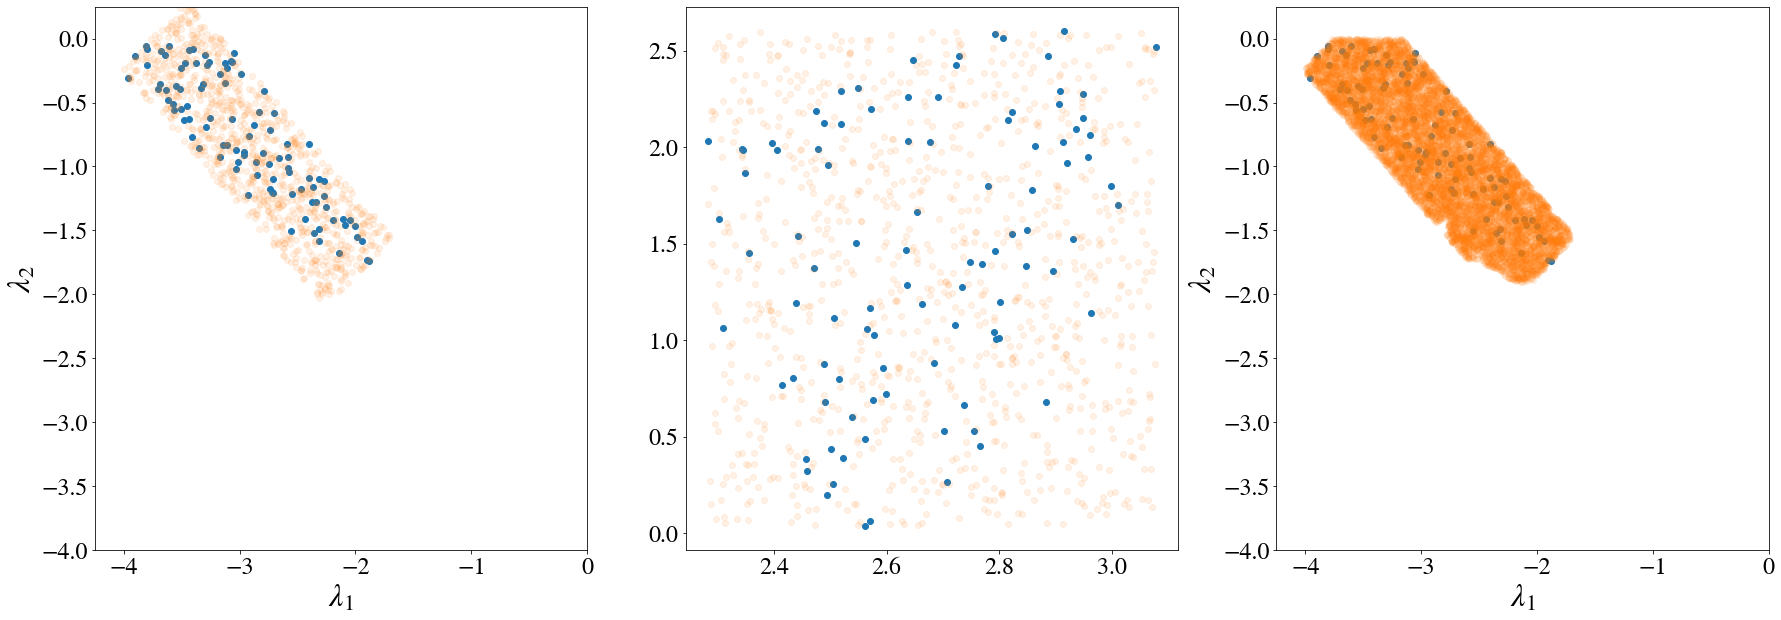
\includegraphics[width=0.95\linewidth]{figures/pde-highd/pde-highd-alt_initial_D2_m100}
\caption{
Generating proposal samples for the two directions informed by solving the 2-D inverse problem, aided by singular-value decompositions and an ad-hoc sampling procedure.
}
\label{fig:pde-highd-2d-study}
\end{figure}

Analogously speaking, we set out to define a computational open cover for the relatively high-probability samples.
In the center panel of Fig~\ref{fig:pde-highd-2d-study}, there are corner-regions of the space we want to avoid wasting samples on as well, so we reject samples that have squared two-norm greater than $0.05$ from their nearest vector--valued sample.
This sampling procedure produces the set shown in orange on the right side of the figure (ten thousand shown to demonstrate coverage).
One thousand of these samples are kept at random and joined with the samples generated from the three other directions.
